% @author Arian Helberg

\chapter{Evaluierung}
Die Synthese von Verzweigungstrukturen wird in den vorangegangenen Kapiteln konzeptionell betrachtet
und in einem Softwareprojekt umgesetzt.
Im Folgendem werden Teilaspekte an einem fortlaufenden Beispiel evaluiert und bewertet.
Diese Aspekte umfassen
\begin{itemize}
    \item das Nutzen von Templates,
    \item die Erstellung und Visualisierung von Verzweigungsstrukturen,
    \item Aufbau einer Baumstruktur,
    \item Extrahierung von Regeln und Mustern,
    \item die Praktikabilität der Algorithmen und
    \item die Umsetzung in einem Programm
\end{itemize}

\subsection*{Templates}
Die Nutzung von Templates als Terminale einer Grammatik findet Anwendung in vielen wissenschaftlichen Arbeiten.
\citeauthor{aliaga_2016} liefert hierzu eine umfassende Übersicht~\cite{aliaga_2016}.
Mit der Verwendung einer allgemeinen Repräsentation mithilfe von \textit{turtle}-Befehlen, wird eine
Wiederverwendbarkeit der genutzten Templates sichergestellt.
Die in dieser Arbeit erstellte Software nutzt ein minimalistisches System zum Einlesen der Templates aus
einer textbasierten Datei, währen die Forschung zur inversen prozeduralen Modellierung den Einsatz von
neuronalen Netzen als vielversprechende Methode Strukturen zu erkennen und Regeln abzuleiten, zeigt.\\
Während neuronale Netze eine Eingabestruktur analysieren und in einer baumähnlichen Struktur organisieren,
knüpft diese Arbeit hier an und nutzt stattdessen aus Praktikabilitätsgründen eine benutzergeführte Anordnung
von Templates zu einer Verzweigungsstruktur.\\~\\
\underline{Beispiel}: Die Template-Zeichenketten haben folgende Form:
\begin{figure}[H]
    \centering
    \begin{csource}
FX
F-FX
F+FX
F[-FX]+FY
F[-FX]FY
F[FX]+FY
F[-FX][FY]+FZ
F[+FX]F[-FY]FZ
    \end{csource}
    \caption{templates.txt}
\end{figure}
\textit{F}, \textit{-}, \textit{+}, \textit{[} und \textit{]} sind dem Turtle-Algorithmus bekannte
Befehlssymbole.
Alle anderen (z.B. \textit{X, Y, Z}) stellen Verzweigungsvariablen dar, um anzuzeigen, an welcher Stelle
der Templatestruktur eine neue Verzweigung abgehen kann.

\subsection*{Erstellung und Visualisierung}
Durch die Ausführung bestimmter \textit{turtle}-Befehle der template-basierten Struktur, wird diese visualisiert.
Darum bietet es sich an, einfache grafische Elemente zu nutzen, um Verzweigungsstrukturen sichtbar zu machen
(z.B. Canvas).
Das Programm nutzt interaktive Elemente (JavaFX Pane) gegenüber staatischen Elementen, um die Strukturen zu zeichnen,
da der Prozess der Erstellung benutzergeführt ist.
So können Elemente genutzt werden, mit denen der Benutzer kommunizieren kann (z.B. klickbare Kreise, farbige
Linien).
So ist es möglich sinierte Verzweigungsstrukturen in einem simplen Arbeitsablauf zu ertstellen.\\~\\
\underline{Beispiel}: Aus dem Erstellen der Verzweigungsstruktur ergibt sich:
\begin{figure}[H]
    \centering
    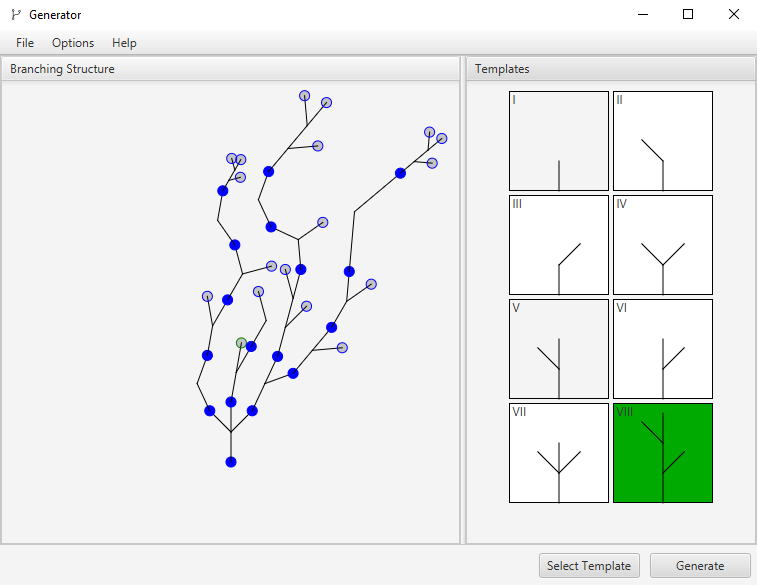
\includegraphics[width=12cm]{../images/evaluierung_inferrieren.png}
    \caption{Grafische Benutzeroberfläche nach der Erstellung der Basisstruktur}
\end{figure}

\subsection*{Aufbau einer Baumstruktur}
Baumähnliche Strukturen eignen sich gut, um Tansformationsparameter und topologische Anordnung von Tempaltes
datenstrukturell zu trennen.
Ansätze zur ganzheitlichen Betrachtung von Eingabestrukturen, also das Einbinden der Transformationen,
und zur Trennung von Transformation und Topologie sind Gegenstand der Forschung.
Das von \citeauthor{benes_2011} vorgestellte System beispielsweise nutz den ganzheitlichen Ansatz, um sog.
\textit{Guides} zu erstellen, welche Teilsysteme der Eingabestruktur beschreiben.
Hier unterscheiden sich Strukturen, die zwar identische Verzweigungen aufweisen, sich aber in Ausprägungen
von Transformationsparametern (z.B. der Winkel von Verzweigungen) unterscheiden.
Auch in der Arbeit~\cite{stava_2010} von \citeauthor{stava_2010} zeigt sich eine Organisation von
"`Clustern"' mit Transformationen, die in eine Signifikanzbewertung einfließen.\\
Auf der anderen Seite zeigen \citeauthor{nishida_2016} und \citeauthor{guo_2020},
dass zum Einen eine seperate Untersuchung der Transformationen mithilfe eines zweiten,
auf seine Aktivität zugeschnittenes, neuronales Netz~\cite{nishida_2016}, zum Anderen dass die meisten
räumlichen Transformationen die Erkennung mittels neuronalem Netz nicht signifikant beeinflussen,
sinnvoll ist.\\~\\
Diese Arbeit legt der Fokus auf die datenstrukturelle Trennung von Transformationen und topologischer
Anordnung und erstellt somit eine Baumstruktur, die Template-Instanzen als Knoten und
räumliche Transformationen als eingehende Kanten darstellt.\\~\\
\underline{Beispiel}: Aus der Eingabestruktur ergibt sich folgender Baum (die räumlichen Transformationen,
die die eingehenden Kanten jedes Knotens darstellen, sind hier nicht visualisiert):
\begin{figure}[H]
    \centering
    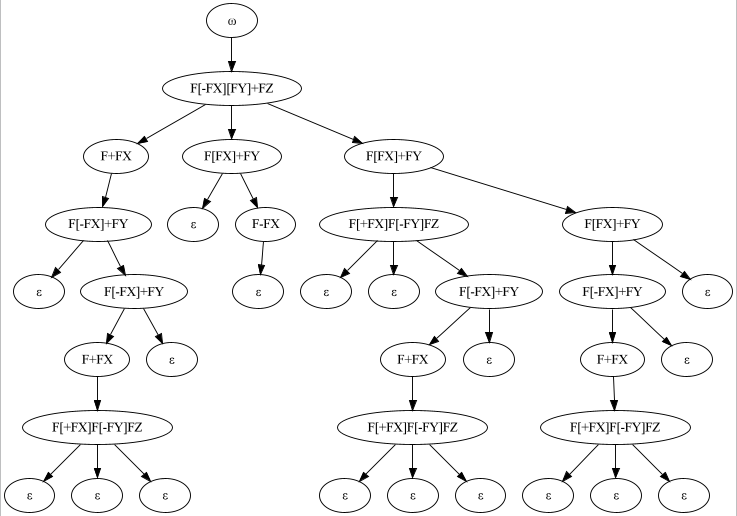
\includegraphics[width=14cm]{../images/evaluierung_inferrieren_baum.png}
    \caption{Baumstruktur der erstellten Verzweigungsstruktur}
\end{figure}

\subsection*{Extrahieren von Regeln und Mustern}
Die in~\ref{alg2} vorgestellte Methodik zum Inferrieren eines L-Systems aus einer Baumstruktur
stellt einen Algorithmus vor, der auf die spezielle Baumstruktur zugeschnitten ist.
Die L-Systeme entsprechen lediglich der Eingabestruktur und beinhalten keine Transformationen.\\~\\
\underline{Beispiel}: Ersetzungssysteme werden über einen JavaFX Dialog visualisiert:
\begin{figure}[H]
    \centering
    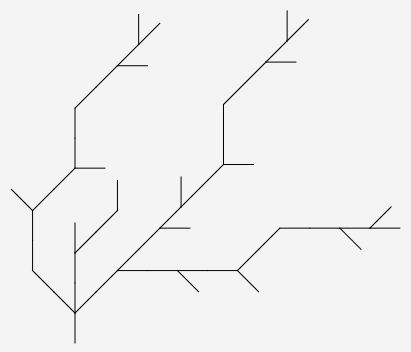
\includegraphics[width=8cm]{../images/evaluierung_inferrieren_lsystem.png}
    \caption{Resultierenden L-System}
\end{figure}
Die Zeichenkettenrepräsentation des L-Systems lautet:
\begin{csource}
LSystem{
    [F, S, A, B, C, D, E, G, H, I, J, K, L, M, N, O, P, Q, R],
    S,
    [S -> A, A -> F[-FB][FC]+FD, B -> F+FE, C -> F[FG]+FH, D -> F[FI]+FJ, E -> F[-FK]+FL, G -> _, H -> F-FM, I -> F[+FN]F[-FO]FP, J -> F[FQ]+FR, K -> _, L -> F[-FF+FF[+F]F[-F]F]+F, M -> _, N -> _, O -> _, P -> F[-FF+FF[+F]F[-F]F]+F, Q -> F[-FF+FF[+F]F[-F]F]+F, R -> _]
}
\end{csource}

Das inferrierte L-System zeigt, dass die Eingabestruktur richtig in eine Grammatik überführt wurde.
